


\subsection{A1 DH Parameters for 3-DOF RRR Puma}

In order to determine the DH Parameter for the 3-DOF Puma we have to follow the steps presented in the tutorial. 

\begin{itemize}
    \item [1.] Identify joint axes; consider i-1 and i
    \item [2.] Identify common perpendicular
    \item [3.] Label frame origin at perpendicular (or intersection)
    \item [4.] Assign $\hat{Z}_i$ along joint axis
    \item [5.] Assign $\hat{X}_i$ along perpendicular;
    if joint axes intersect, orthogonal to the axes plane
    \item [6.] Complete frame by adding Y axis (right-hand-rule)
    \item [7.] Assign {0} to match {1}
    \item [8.] Choose end-effector frame {n}
\end{itemize}
Most of the steps were already performed in the Puma Robot sketch below. The x-axis and y-axis were already assigned for all joints and the $\hat{Z}_i$ can be determined through the right hand rule to be pointing into the schematic. Therefore positive change in angle is clockwise. 

\begin{figure} [H]
   \begin{center}
        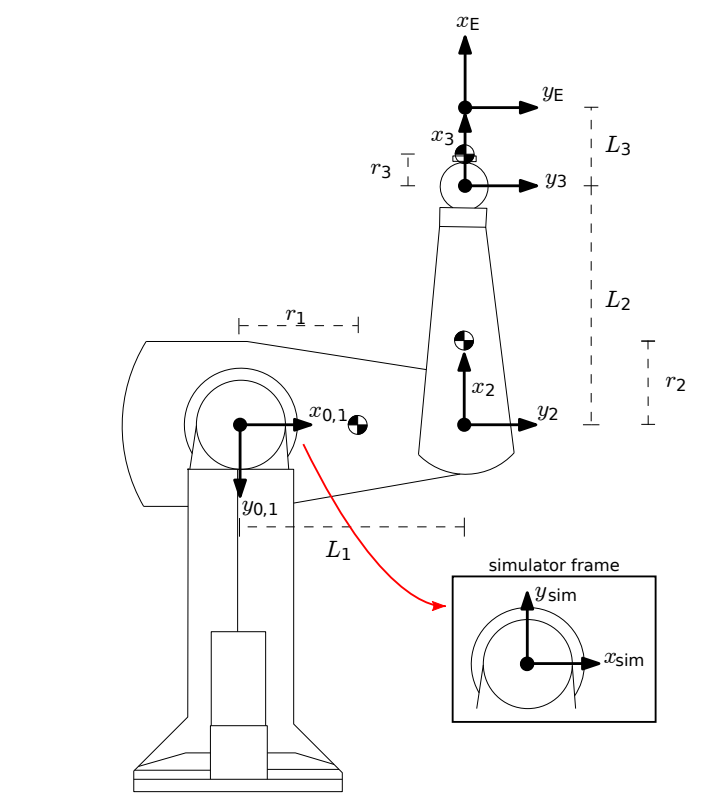
\includegraphics[width=0.5\textwidth]{SRC/PumaRoboter.PNG}
   \end{center}
  \caption{3-DOF RRR Puma depiction from the task sheet.}
  \label{fig:TaskPuma}
\end{figure}

To fill the DH parameter in the table, the following in the tutorial presented steps must be followed.

\begin{itemize}
    \item $\alpha_i$ = the angle between $\hat{Z_i}$ and $\hat{Z}_{i+1}$ measured about $\hat{X}_i$
    \item $a_i$ = the distance from $\hat{Z}_i$ and $\hat{Z}_{i+1}$ measured along $\hat{X}_i$
    \item $d_i$ = the distance from $\hat{X}_{i-1}$ and $\hat{X}_{i}$ measured along $\hat{Z}_i$
    \item $\theta_i$ = the angle between $\hat{X}_{i-1}$ and $\hat{X}_{i}$ measured about $\hat{Z}_i$
\end{itemize}

\begin{table}[h]
    \centering
    \begin{tabular}{ |p{1cm}|p{1cm}|p{1cm}|p{1cm}|p{1.5cm}|  } 
        \hline 
       $i$ & $\alpha_{i-1}$ & $a_{i-1}$ &$d_i$ & $\theta_i$\\
        \hline
        \hline
       1 &  0 & 0 & 0 & $q_1$\\
        \hline
         2 &  0 & $l_1$ & 0 & $q_2-\frac{\pi}{2}$\\
          \hline
         3 &  0 &$l_2$& 0 & $q_3$\\
         \hline
         4(E) &  0 & $l_3$ & 0 & 0\\
        \hline
    \end{tabular}
    \caption{DH Parameters.}
    \label{Table:DH}
\end{table}

As one can clearly see in Figure \ref{fig:TaskPuma}, when choosing x0=x1 and y0=y1 and following the right-hand rule, all $\hat{Z}$ axes are aligned. Therefore the column of the $\alpha_i$'s that represent the angle of the $\hat{Z}_i$'s to each other is zero. The distance between the $\hat{Z}_i$'s is obviously the different lengths of the parts connecting the joints. As $\hat{Z}_0 = \hat{Z}_1$ ; $a_0$=0 and the others $l_1$, $l_2$ and $l_3$ respectively. As all joints have the same oriented $\hat{Z}$ it is also clear that the distance along $\hat{Z}_i$ of the $\hat{X}_i$ is always zero. The angle between $\hat{X}_i$ and $\hat{X}_{i-1}$ represents the angle between the joints. That's why joint 3 compared to the end effector is 0,  $\theta_1=q_1$ and $\theta_3=q_3$. As in the neutral configuration the second joint is rotated by $-\frac{\pi}{2}$ about $\hat{Z}_2$ (negative because the $\hat{Z}_i$'s are pointing into the image according to the right-hand rule), $\theta_2=q_2-\frac{\pi}{2}$.




\subsection{A2 Transformation between frames}
\begin{equation}
   \prescript{i-1}{i}{T} = \begin{pmatrix} 
   c\theta_i & -s\theta_i & 0 & a_{i-1}\\
   s\theta_i\cdot c\alpha_{i-1} & c\theta_i\cdot c\alpha_{i-1}& -s\alpha_{i-1}& -s\alpha_{i-1}\cdot d_i\\
   s\theta_i\cdot s\alpha_{i-1}& c\theta_i\cdot s\alpha_{i-1} &c\alpha_{i-1}&  c\alpha_{i-1}\cdot d_i       \\
   0 & 0 & 0 & 1\end{pmatrix}
   \label{eq:Transform}
\end{equation}
Above is depicted the general formula for the individual transformation matrices. 
When we now insert the $\theta_i$'s according to the definition in Table \ref{Table:DH}, we get a -$\frac{\pi}{2}$ shift in all terms that include $\theta_2$. So the $\sin$ terms including $\theta_2$ become $-\cos$ and $\cos$ terms including $\theta_2$ become $\sin$. So inserting the values from Table \ref{Table:DH} in Equation \ref{eq:Transform}, brings the following four transformation matrices. 

\begin{equation}
   \prescript{0}{1}{T} = \begin{pmatrix} 
  c_1 & -s_1 & 0 & 0\\
   s_1 & c_1 & 0& 0\\
   0& 0 & 1 &  0       \\
   0 & 0 & 0 & 1\end{pmatrix}
   \label{eq:T01}
\end{equation}

\begin{equation}
   \prescript{1}{2}{T} = \begin{pmatrix} 
  s_2 & c_2 & 0 & l_1\\
   -c_2 & s_2 & 0& 0\\
   0& 0 & 1 &  0       \\
   0 & 0 & 0 & 1\end{pmatrix}
   \label{eq:T12}
\end{equation}

\begin{equation}
   \prescript{2}{3}{T} = \begin{pmatrix} 
  c_3 & -s_3 & 0 & l_2\\
   s_3 & c_3 & 0& 0\\
   0& 0 & 1 &  0       \\
   0 & 0 & 0 & 1\end{pmatrix}
   \label{eq:T23}
\end{equation}

\begin{equation}
   \prescript{3}{E}{T} = \begin{pmatrix} 
  1 & 0 & 0 & l_3\\
   0 & 1 & 0& 0\\
   0& 0 & 1 &  0       \\
   0 & 0 & 0 & 1\end{pmatrix}
   \label{eq:T34}
\end{equation}


\begin{equation}
   \prescript{0}{E}{T} = \prescript{0}{1}{T} \cdot \prescript{1}{2}{T} \cdot \prescript{2}{3}{T} \cdot \prescript{3}{E}{T}
   \label{eq:tsum}
\end{equation}

\begin{equation}
   \prescript{0}{2}{T} = \prescript{0}{1}{T} \cdot \prescript{1}{2}{T}
\end{equation}

\begin{equation}
   \prescript{0}{2}{T} =\begin{pmatrix} 
  c_1 & -s_1 & 0 & 0\\
   s_1 & c_1 & 0& 0\\
   0& 0 & 1 &  0       \\
   0 & 0 & 0 & 1\end{pmatrix} \cdot \begin{pmatrix} 
  s_2 & c_2 & 0 & l_1\\
   -c_2 & s_2 & 0& 0\\
   0& 0 & 1 &  0       \\
   0 & 0 & 0 & 1\end{pmatrix} 
   \label{eq:tsum}
\end{equation}

\begin{equation}
   \prescript{0}{2}{T} = \begin{pmatrix} 
  c_1 \cdot s_2 + c_2  \cdot s_1 & c_1 \cdot c_2 -s_1 \cdot s_2 & 0 & c_1 \cdot l_1\\
   s_1 \cdot s_2 - c_1 \cdot c_2 &  s_1 \cdot c_2 + s_2 \cdot c_1 & 0& s_1 \cdot l_1\\
   0& 0 & 1 &  0       \\
   0 & 0 & 0 & 1\end{pmatrix}
\end{equation}

According to the following sin and cos sum formulas: 

\begin{equation}
  sin(\alpha \pm \beta)= sin(\alpha) cos(\beta) \pm cos(\alpha)sin(\beta)
\end{equation}

\begin{equation}
  cos(\alpha \pm \beta)= cos(\alpha) cos(\beta) \mp sin(\alpha)sin(\beta)
\end{equation}

the equation can be simplified, where $c_{12}$ refers to $cos(q_1+q_2)$ and $s_{12}$ refers to $sin(q_1+q_2)$.

\begin{equation}
   \prescript{0}{2}{T} = \begin{pmatrix} 
  s_{12} & c_{12} & 0 & c_1 \cdot l_1\\
   -c_{12} & s_{12} & 0& s_1 \cdot l_1\\
   0& 0 & 1 &  0       \\
   0 & 0 & 0 & 1\end{pmatrix}
\end{equation}

Analogously $ \prescript{0}{3}{T}$ can be calculated. 

\begin{equation}
   \prescript{0}{3}{T} = \prescript{0}{2}{T} \cdot \prescript{2}{3}{T}
\end{equation}

\begin{equation}
   \prescript{0}{3}{T} = \begin{pmatrix} 
  s_{12} & c_{12} & 0 & c_1 \cdot l_1\\
   -c_{12} & s_{12} & 0& s_1 \cdot l_1\\
   0& 0 & 1 &  0       \\
   0 & 0 & 0 & 1\end{pmatrix} \cdot \begin{pmatrix} 
  c_3 & -s_3 & 0 & l_2\\
   s_3 & c_3 & 0& 0\\
   0& 0 & 1 &  0       \\
   0 & 0 & 0 & 1\end{pmatrix} 
   \label{eq:tsum}
\end{equation}

\begin{equation}
   \prescript{0}{3}{T} = \begin{pmatrix} 
  s_{123} & c_{123} & 0 & c_1 \cdot l_1 + s_{12} \cdot l_2\\
   - c_{123} & s_{123} & 0& s_1 \cdot l_1 - c_{12} \cdot l_2\\
   0& 0 & 1 &  0       \\
   0 & 0 & 0 & 1\end{pmatrix}
\end{equation}

\begin{equation}
   \prescript{0}{E}{T} = \prescript{0}{3}{T} \cdot \prescript{3}{E}{T}
\end{equation}

\begin{equation}
   \prescript{0}{E}{T} = \begin{pmatrix} 
  s_{123} & c_{123} & 0 & c_1 \cdot l_1 + s_{12} \cdot l_2\\
   - c_{123} & s_{123} & 0& s_1 \cdot l_1 - c_{12} \cdot l_2\\
   0& 0 & 1 &  0       \\
   0 & 0 & 0 & 1\end{pmatrix} \cdot \begin{pmatrix} 
  1 & 0 & 0 & l_3\\
   0 & 1 & 0& 0\\
   0& 0 & 1 &  0       \\
   0 & 0 & 0 & 1\end{pmatrix}
   \label{eq:tsum}
\end{equation}

\begin{equation}
   \prescript{0}{E}{T} = \begin{pmatrix} 
  s_{123} & c_{123} & 0 & c_1 \cdot l_1 + s_{12} \cdot l_2 + s_{123} \cdot l_3\\
   -c_{123} & s_{123} & 0& s_1 \cdot l_1 - c_{12} \cdot l_2 - c_{123} \cdot l_3\\
  0& 0 & 1 &  0       \\
   0 & 0 & 0 & 1\end{pmatrix}
   \label{eq:TEFINAL}
\end{equation}

This matrix can be easily tested with the simulator software.
For the configuration $q_{test1}$=($q_1$, $q_2$, $q_3$)=(0, $\frac{\pi}{2},0)$ we expect the Puma to be fully extended in x direction. So the resulting x translation should be the length of the puma and the y translation 0. 

\begin{equation}
   \prescript{0}{E}{T}(q_{test1}) = \begin{pmatrix} 
  1 & 0 & 0 & 1 \cdot l_1 + 1 \cdot l_2 + 1 \cdot l_3\\
   0 & 1 & 0& 0 \cdot l_1 - 0 \cdot l_2 - 0 \cdot l_3\\
   0& 0 & 1 &  0       \\
   0 & 0 & 0 & 1\end{pmatrix}
\end{equation}

The translation can be looked up from the last column of the matrix. Therefore it would be $l_1+ l_2 +l_3$ on the x-axis and 0 on the y-axis. Which fulfills the expectation. \newline
Another test configuration $q_{test2}$=($q_1$, $q_2$, $q_3$)=($-\frac{\pi}{4}$, $\frac{\pi}{2}$,0). In this configuration the puma is extended at an angle of 45°. The x coordinate should be sin/cos(45°)=$\frac{\sqrt{2}}{2}\cdot (l_1 + l_2+ l_3)$ and y=-$\frac{\sqrt{2}}{2}\cdot (l_1 + l_2+ l_3)$, as the simulator frame has a mirrored y axis.

\begin{equation}
   \prescript{0}{E}{T}(q_{test2}) = \begin{pmatrix} 
  \frac{\sqrt{2}}{2} & -\frac{\sqrt{2}}{2} & 0 & \frac{\sqrt{2}}{2} \cdot l_1 + \frac{\sqrt{2}}{2} \cdot l_2 + \frac{\sqrt{2}}{2} \cdot l_3\\
   \frac{\sqrt{2}}{2} & \frac{\sqrt{2}}{2} & 0& -\frac{\sqrt{2}}{2} \cdot l_1 - \frac{\sqrt{2}}{2} \cdot l_2 - \frac{\sqrt{2}}{2} \cdot l_3\\
   0& 0 & 1 &  0       \\
   0 & 0 & 0 & 1\end{pmatrix}
\end{equation}

In this case the transformation matrix delivers the expected results as well.


If we wanted to align our base frame (x0,1/y0,1) with the simulator frame, we would choose x0,1 and y0,1 in its orientation and would only have a rotation along the $\hat{X}_1$. So that the adjusted DH table and the transformation matrix $\prescript{0}{E}{T}$ would be as follows to mirror the base frame y-axis.

\begin{table}[H]
    \centering
    \begin{tabular}{ |p{1cm}|p{1cm}|p{1cm}|p{1cm}|p{1.5cm}|  } 
        \hline 
       $i$ & $\alpha_{i-1}$ & $a_{i-1}$ &$d_i$ & $\theta_i$\\
        \hline
        \hline
       1 &  0 & 0 & 0 & $q_1$\\
        \hline
         2 &  $-\pi$ & $l_1$ & 0 & $q_2-\frac{\pi}{2}$\\
          \hline
         3 &  0 &$l_2$& 0 & $q_3$\\
         \hline
         4(E) &  0 & $l_3$ & 0 & 0\\
        \hline
    \end{tabular}
    \caption{DH parameter if orientated according to the simulator frame.}
    \label{Table:DH_simFrame}
\end{table}

\begin{equation}
   \prescript{0}{E}{T} = \begin{pmatrix} 
  s_{-123} & c_{-123} & 0 & c_1 \cdot l_1 + s_{12} \cdot l_2 + s_{123} \cdot l_3\\
   c_{-123} & -s_{-123} & 0& - s_1 \cdot l_1 + c_{12} \cdot l_2 + c_{123} \cdot l_3\\
  0& 0 & 1 &  0       \\
   0 & 0 & 0 & 1\end{pmatrix}
\end{equation}

\newline 
\newline
As not otherwise stated in the task we gonna proceed using the original $\prescript{0}{E}{T}$ (see Equation \ref{eq:TEFINAL}) and DH (see Table \ref{Table:DH}) parameters in the following.

\subsection{A3 - End effector position in operational space}
As seen in the previous subtask, the translational x and y components of the F vector can be taken from the first two rows of the last column of $\prescript{0}{E}{T}$.
For the angle alpha we only need to sum up the angle $\theta_i$ as those describe the angular translation between the starting joint and the endeffector. The resulting F is as follows. 

\begin{equation}
    F(q) = \begin{pmatrix} 
  c_1 \cdot l_1 + s_{12} \cdot l_2 + s_{123} \cdot l_3\\
  s_1 \cdot l_1 - c_{12} \cdot l_2 - c_{123} \cdot l_3\\
   q_1 + q_2 - \frac{\pi}{2} + q_3   \end{pmatrix}
   \label{eq:fformula}
\end{equation}


We can test this once again with the Stanford Puma simulator, by calculating F according to Equation \ref{eq:fformula} and comparing it to the simulator results.



\begin{equation}
    F(0,\frac{\pi}{2},0) = \begin{pmatrix} 
    l_1 + l_2 + l_3\\
    0 \\
    0  \end{pmatrix}
\end{equation}

\begin{equation}
    F(-\frac{\pi}{4},\frac{\pi}{2},0) = \begin{pmatrix} 
    \frac{\sqrt{2}}{2}\cdot (l_1 + l_2 + l_3)\\
    -\frac{\sqrt{2}}{2}\cdot (l_1 + l_2 + l_3) \\
    -\frac{\pi}{4}  \end{pmatrix}
\end{equation}

\begin{equation}
    F(-\frac{3\pi}{4},\frac{\pi}{2},0) = \begin{pmatrix} 
    -\frac{\sqrt{2}}{2}\cdot (l_1 + l_2 + l_3)\\
    -\frac{\sqrt{2}}{2}\cdot (l_1 + l_2 + l_3) \\
    -\frac{3\pi}{4}  \end{pmatrix}
\end{equation}

Those results are all equivalent in the puma simulator (with respect to the mirrored y-axis frame) which concludes the testing of the calculated F matrix. 

\subsection{A4 - Compute the endeffector jacobian}

The Jacobian of F can be computed by deriving each of its rows by all of the states ($q_1$, $q_2$, $q_3$). So the Jacobian is defined in our case as follows. ($F_i$ refers to the i-th row of $F(q)$).



\begin{equation}
    J(q) = \begin{pmatrix} 
    \frac{\delta F_1}{\delta q_1}&  \frac{\delta F_1}{\delta q_2}&  \frac{\delta F_1}{\delta q_3}\\
    \frac{\delta F_2}{\delta q_1}&  \frac{\delta F_2}{\delta q_2}&  \frac{\delta F_2}{\delta q_3} \\
    \frac{\delta F_3}{\delta q_1}&  \frac{\delta F_3}{\delta q_2}&  \frac{\delta F_3}{\delta q_3}  \end{pmatrix}
\end{equation}

As the angles have no factor in front of the the derivatives can be calculated trivially


\begin{equation}
    J(q)  = \begin{pmatrix} 
  -s_1 \cdot l_1 + c_{12} \cdot l_2 + c_{123} \cdot l_3
  &  c_{12} \cdot l_2 + c_{123} \cdot  l_3& l_3\cdot c_{123}
  \\
   c_1 \cdot l_1 + s_{12} \cdot l_2 + s_{123} \cdot l_3 &  s_{12} \cdot l_2 + s_{123} \cdot l_3&  s_{123} \cdot l_3 \\ 
   1 & 1 & 1\end{pmatrix}
   \label{eq:Jmatrix}
\end{equation}


\subsection{A5 - Understanding the jacobian matrix and pose singularities}

When calculating the following tasks it is important to keep in mind that the base frame y-axis (y0,1) is pointing downwards. So negative y change is an upward movement and positive y a downward movement (as it is counterintuitive).

\subsubsection{i}
\textbf{$q_1=(0, 0 , -\frac{\pi}{2}$})
\newline 
Inserting $q_1$ in Equation \ref{eq:fformula} to get $F(q_1)$.

\begin{equation}
    x(q_1) = F(q_1) = \begin{pmatrix} 
   l_1 + 0 - l_3\\
   0 - l_2 + 0\\
  -\frac{\pi}{2} -\frac{\pi}{2}  \end{pmatrix} = \begin{pmatrix} 
   l_1 - l_3\\
 -l_2 \\
  -\pi  \end{pmatrix}
\end{equation}


Inserting $q_1$ in Equation \ref{eq:Jmatrix} to get $J(q_1)$.

\begin{equation}
    J(q_1) = \begin{pmatrix} 
  l_2&l_2&0\\
  l_1-l_3& -l_3& -l_3\\
  1  & 1 & 1\end{pmatrix}
\end{equation}

To get the velocities in the x coordinate frame we need to apply the following formula.

\begin{equation}
    \dot{x}(q_1)=J(q_1)\cdot \dot{q}
\end{equation}

Für $\dot{q}=(1\ 0\ 0)^T$:

\begin{equation}
    \dot{x}_1(q_1)=J(q_1)\cdot (1\ 0\ 0)^T = \begin{pmatrix} 
  l_2\\
  l_1-l_3\\
  1\end{pmatrix}
\end{equation}

Für $\dot{q}=(0\ 1\ 0)^T$:

\begin{equation}
    \dot{x}_2(q_1)=J(q_1)\cdot (0\ 1\ 0)^T = \begin{pmatrix} 
  l_2\\
  -l_3\\
  1\end{pmatrix}
\end{equation}

Für $\dot{q}=(0\ 0\ 1)^T$:

\begin{equation}
    \dot{x}_3(q_1)=J(q_1)\cdot (0\ 1\ 0)^T = \begin{pmatrix} 
  0\\
  -l_3\\
  1\end{pmatrix}
\end{equation}


\begin{figure} [H]
   \begin{center}
        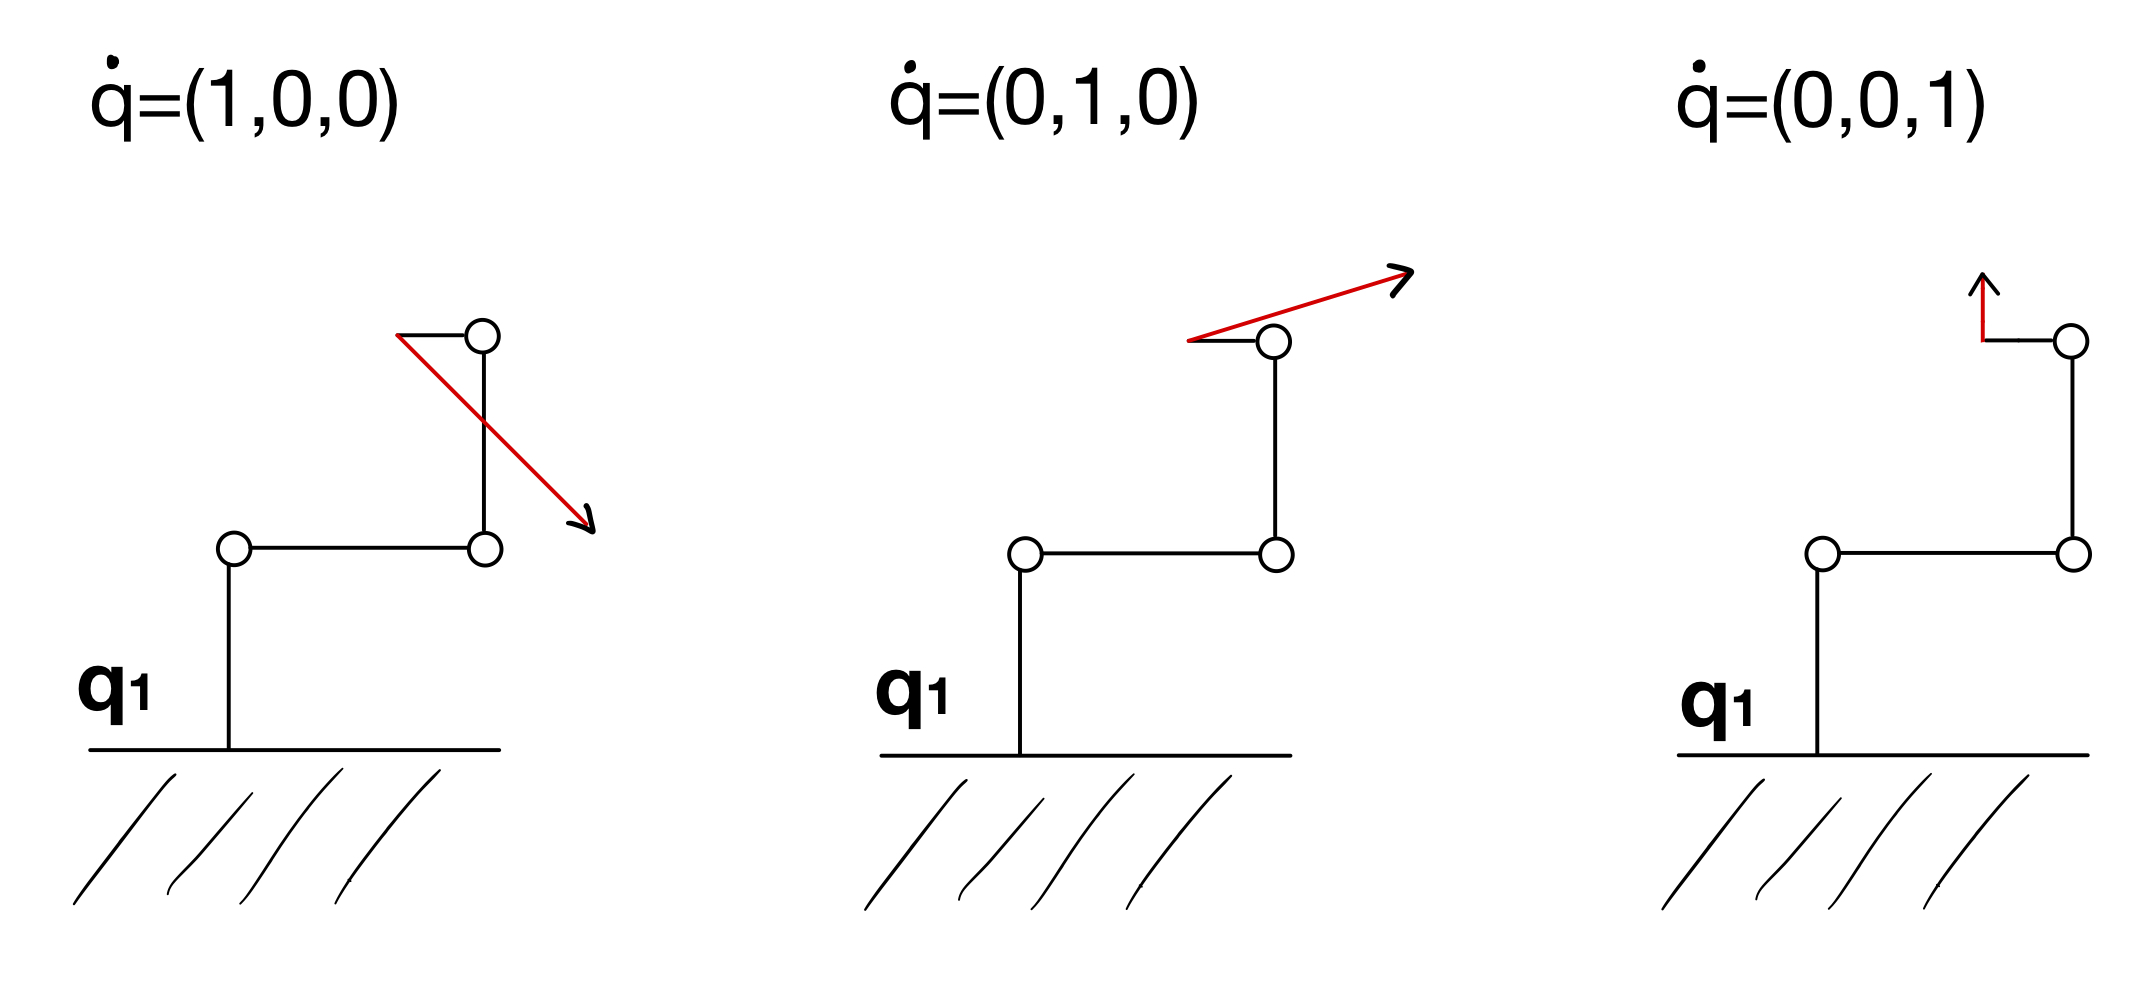
\includegraphics[width=0.6\textwidth]{SRC/q_1_joints.JPEG}
   \end{center}
  \caption{Effect of each joint on translational velocities for initial configuration $q_1$.}
  \label{fig:q1}
\end{figure}

As we can see from the calculation of the impact of each joint on the x frame velocities $\dot{x}_1$, $\dot{x}_2$, $\dot{x}_3$ and the sketch representing it, the puma in this configuration is controllable in each direction. This can be seen directly in the Jacobian J($q_1$), as none of its rows is close to or equal to zero. 

\subsubsection{ii}
\textbf{$q_2=(-\frac{\pi}{2}, \frac{\pi}{2}$ , 0.1})
\newline 
Inserting $q_2$ in Equation \ref{eq:fformula} to get $F(q_2)$.
\begin{equation}
    F(q_2) = \begin{pmatrix} 
   sin(0.1)\cdot l_3\\
  -l_1 - l_2 - cos(0.1)\cdot l_3\\
  0.1-\frac{\pi}{2}  \end{pmatrix}
\end{equation}
Inserting $q_2$ in Equation \ref{eq:Jmatrix} to get $J(q_2)$.
\begin{equation}
    J(q_2) = \begin{pmatrix} 
   l_1 + l_2 + cos(0.1)\cdot l_3& l_2 + cos(0.1)\cdot l_3& cos(0.1)\cdot l_3\\
  sin(0.1)\cdot l_3& sin(0.1)\cdot l_3& sin(0.1)\cdot l_3\\
  1  & 1 & 1\end{pmatrix}
\end{equation}

\begin{equation}
    J(q_2) \approx \begin{pmatrix} 
   l_1 + l_2 + 0.99\cdot l_3& l_2 + 0.99\cdot l_3& 0.99\cdot l_3\\
  0.1\cdot l_3& 0.1\cdot l_3& 0.1\cdot l_3\\
  1  & 1 & 1\end{pmatrix}
\end{equation}


Für $\dot{q}=(1\ 0\ 0)^T$:

\begin{equation}
    \dot{x}(q_2)=J(q_2)\cdot (1\ 0\ 0)^T = \begin{pmatrix} 
  l_1 + l_2 + 0.99\cdot l_3\\
  0.1\cdot l_3\\
  1\end{pmatrix}
\end{equation}

Für $\dot{q}=(0\ 1\ 0)^T$:

\begin{equation}
    \dot{x}(q_2)=J(q_2)\cdot (0\ 1\ 0)^T = \begin{pmatrix} 
  l_2+0.99 \cdot l_3\\
  0.1 \cdot l_3\\
  1\end{pmatrix}
\end{equation}

Für $\dot{q}=(0\ 0\ 1)^T$:

\begin{equation}
    \dot{x}(q_2)=J(q_2)\cdot (0\ 1\ 0)^T = \begin{pmatrix} 
  0.99\cdot l_3\\
  0.1 \cdot l_3\\
  1\end{pmatrix}
\end{equation}

\begin{figure} [H]
   \begin{center}
        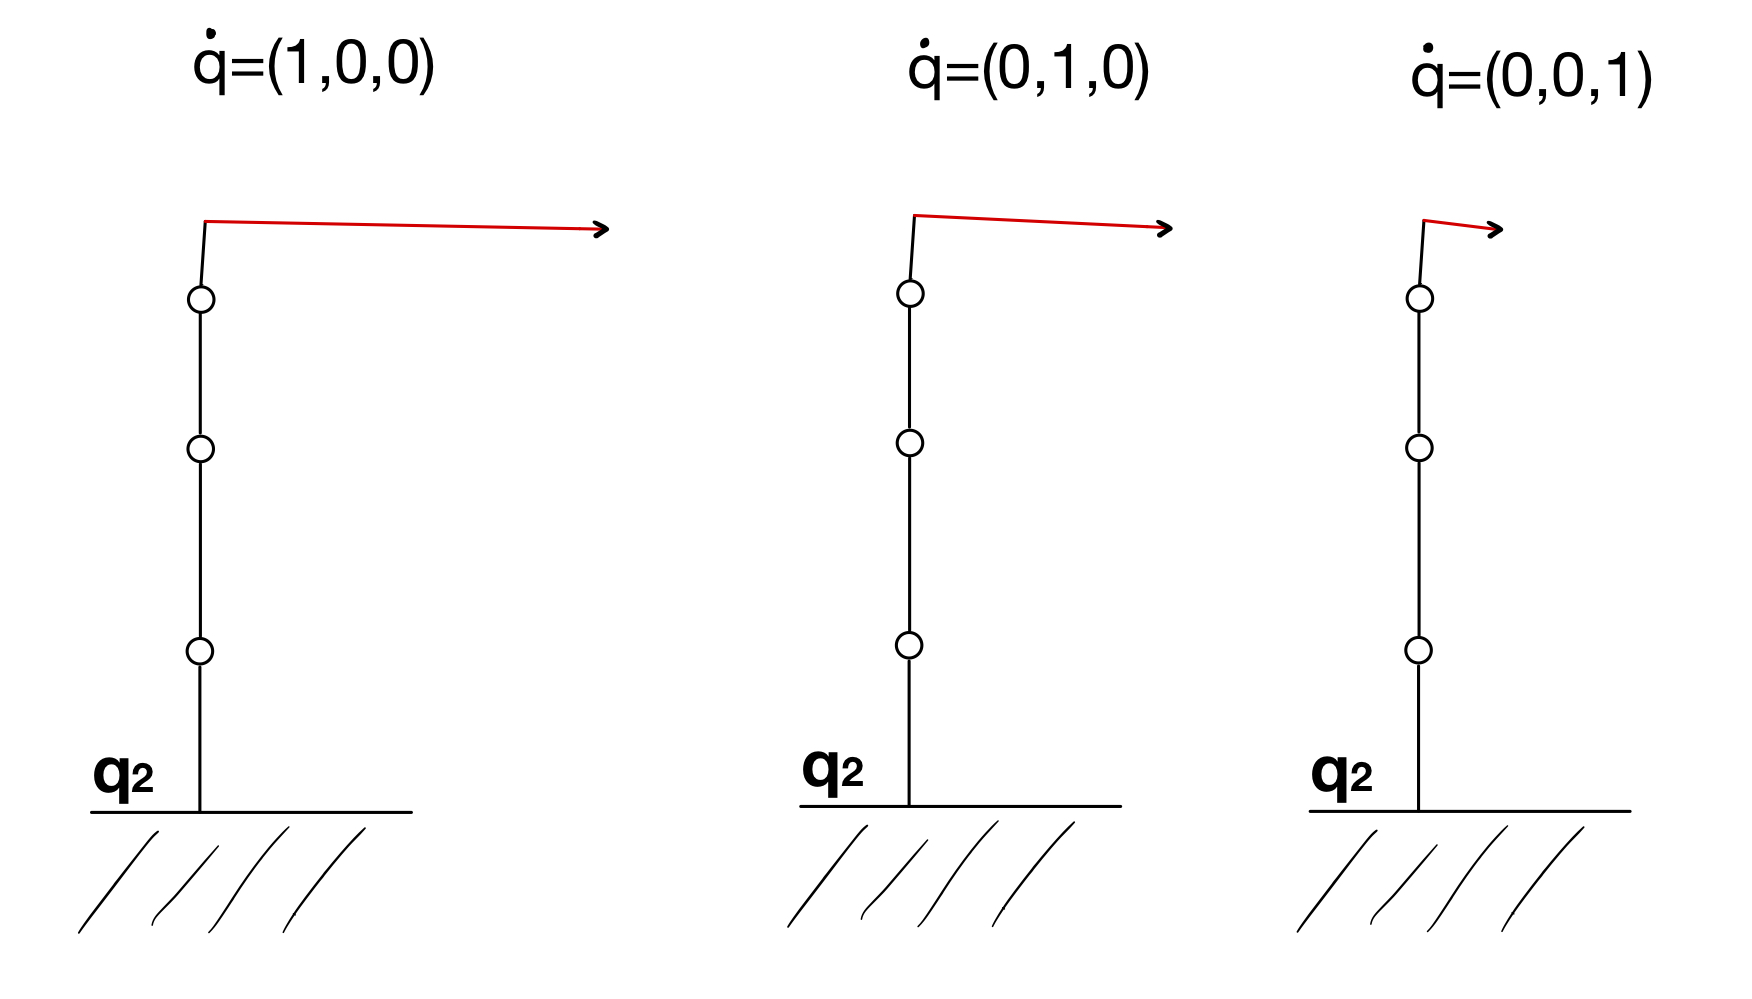
\includegraphics[width=0.6\textwidth]{SRC/q_2_joints.JPEG}
   \end{center}
  \caption{Effect of each joint on translational velocities for initial configuration $q_2$.}
  \label{fig:q2}
\end{figure}

For configuration $q_2$ we can see that we are close to a singularity. The second row of the Jacobian J($q_2$) is getting close to zero and the y-components of the x frame velocities is therefore also getting smaller. However we are not at a singularity as we can still impact the y velocity component a little bit by the change in joint angles.


\subsubsection{iii}
\textbf{$q_2=(-\frac{\pi}{2}, \frac{\pi}{2}$ , 0})
\newline 
Inserting $q_3$ in Equation \ref{eq:fformula} to get $F(q_3)$.
\begin{equation}
    F(q_3) = \begin{pmatrix} 
   0 + 0 - 0\\
  -l_1 - l_2 - l_3\\
  -\frac{\pi}{2} + \frac{\pi}{2} - \frac{\pi}{2} +  0\end{pmatrix}= \begin{pmatrix} 
   0\\
   - l_1 - l_2 - l_3\\
  -\frac{\pi}{2}  \end{pmatrix}
\end{equation}
Inserting $q_3$ in Equation \ref{eq:Jmatrix} to get $J(q_3)$.
\begin{equation}
    J(q_3) = \begin{pmatrix} 
   l_1 + l_2 + l_3 & l_2 +l_3& l_3 \\
  0&0&0\\
  1  & 1 & 1\end{pmatrix}
\end{equation}

Für $\dot{q}=(1\ 0\ 0)^T$:

\begin{equation}
    \dot{x}(q_3)=J(q_3)\cdot (1\ 0\ 0)^T = \begin{pmatrix} 
  l_1+ l_2\\
  0\\
  1\end{pmatrix}
\end{equation}

Für $\dot{q}=(0\ 1\ 0)^T$:

\begin{equation}
    \dot{x}(q_3)=J(q_3)\cdot (0\ 1\ 0)^T = \begin{pmatrix} 
  l_2+l_3\\
  0\\
  1\end{pmatrix}
\end{equation}

Für $\dot{q}=(0\ 0\ 1)^T$:

\begin{equation}
    \dot{x}(q_3)=J(q_3)\cdot (0\ 1\ 0)^T = \begin{pmatrix} 
  l_3\\
  0\\
  1\end{pmatrix}
\end{equation}

\begin{figure} [H]
   \begin{center}
        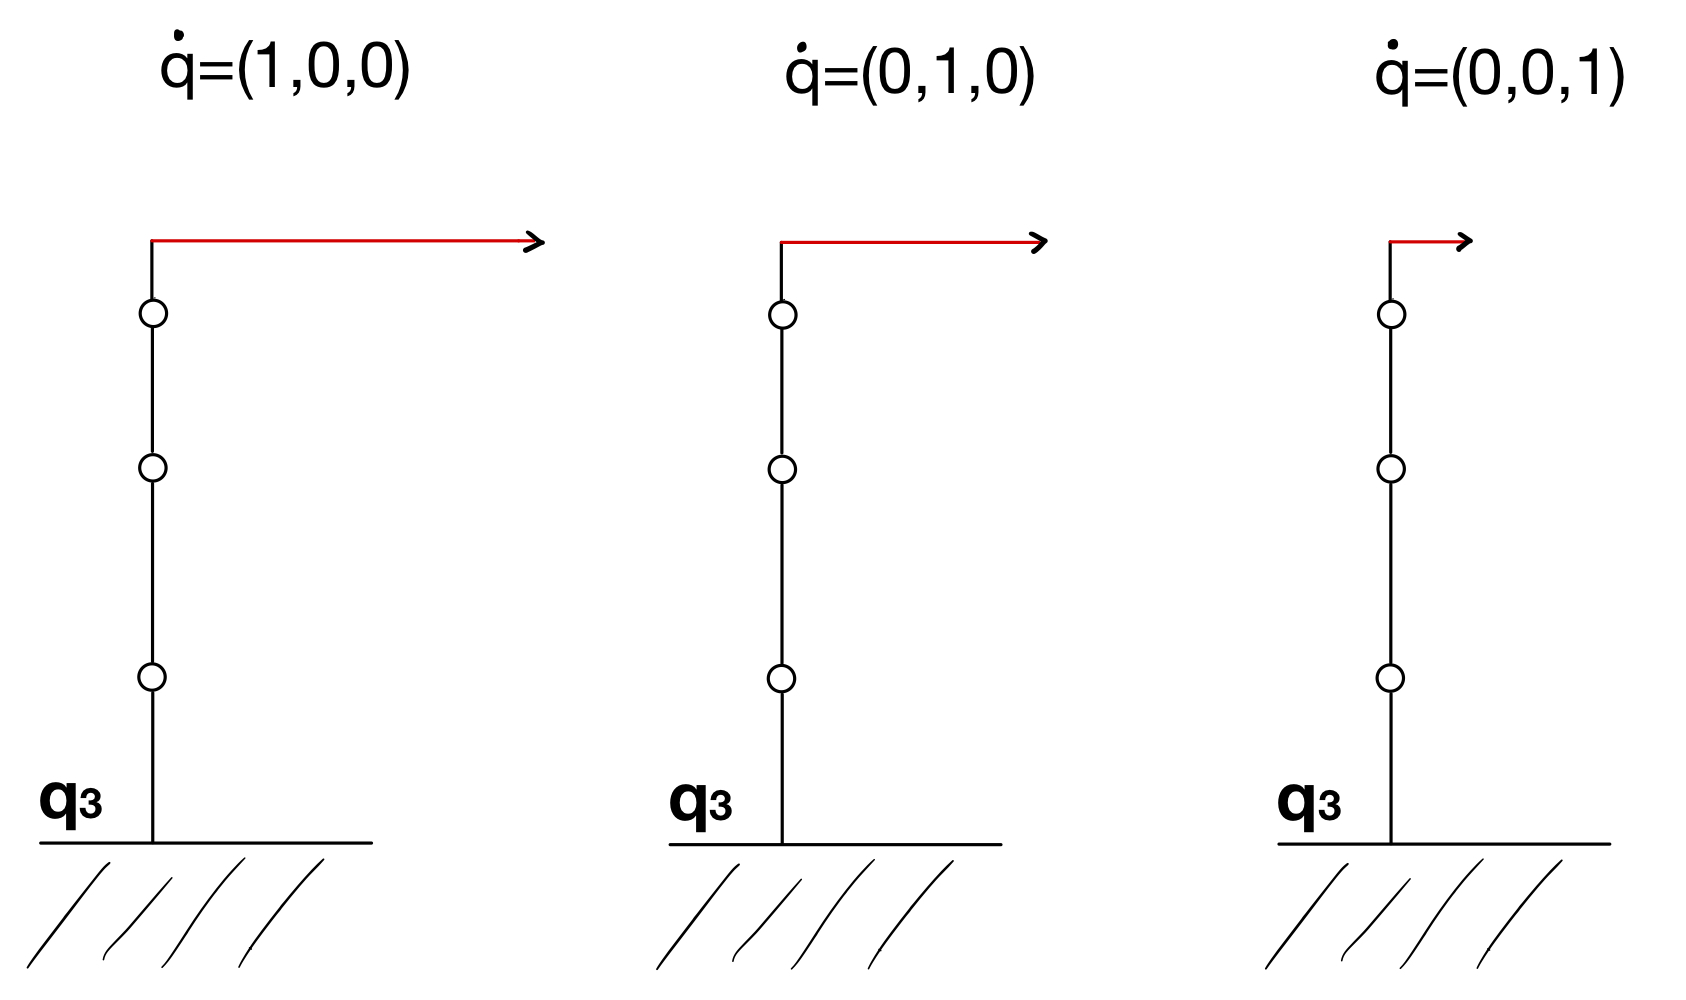
\includegraphics[width=0.6\textwidth]{SRC/q_3_joints.JPEG}
   \end{center}
  \caption{Effect of each joint on translational velocities for initial configuration $q_2$.}
  \label{fig:q3}
\end{figure}

Configuration $q_3$ is clearly a singular case as the second row of the Jacobian J($q_3$) is zero and none of the changes in the joint angles have an impact on the y-axis velocity. 